\documentclass{standalone}
\usepackage{tikz}
\usepackage{pgfplots}
\pgfplotsset{compat=newest}
\usepackage{amsmath}
\usepackage[american]{circuitikz}
\usepackage{cmbright}

\ctikzset{bipoles/resistor/height=0.2, bipoles/resistor/width=0.6}

\definecolor{myred}{RGB}{170,0,0}
\definecolor{myblue}{RGB}{0,0,220}
\definecolor{mygreen}{RGB}{0,150,0}
\definecolor{myorange}{RGB}{255,127,0}
\definecolor{mybrown}{RGB}{150,75,0}

\begin{document}
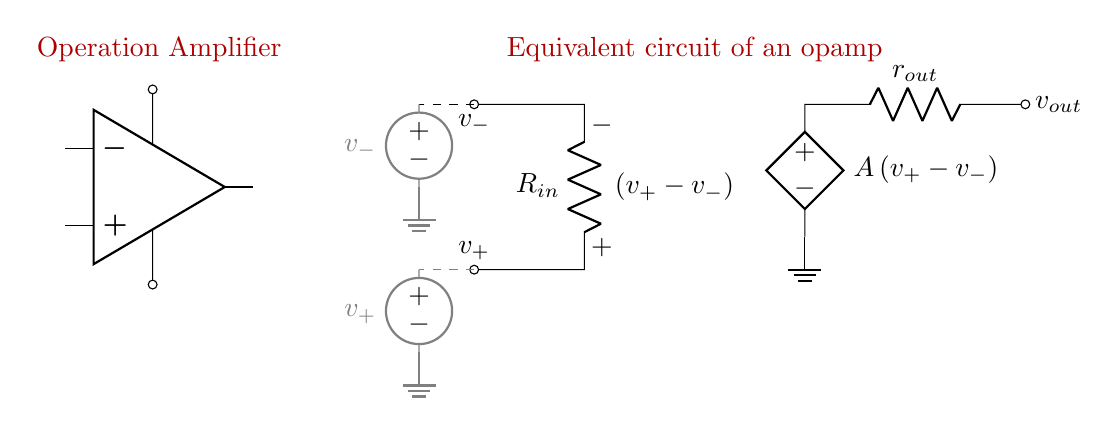
\begin{tikzpicture}
    \begin{scope}[scale=0.7]
        % Title
        \node[anchor=center, color=myred] at (0, 2.5) {Operation Amplifier};
        \draw (0, 0) node[op amp] (OpAmp) {};
        \draw (OpAmp.up) 
            to[short, -o] ++(0, 1.0);
        \draw (OpAmp.down) 
            to[short, -o] ++(0, -1.0);
    \end{scope}
    \begin{scope}[xshift=4cm, scale=0.7]
        % Title
        \node[anchor=center, color=myred] at (4, 2.5) {Equivalent circuit of an opamp};
        \draw (0, 1.5)
            node[anchor=north] {$v_{-}$}
            to[short, o-] ++(2.0, 0)
            to[R, v^<={$(v_{+} - v_{-})$}, l_={$R_{in}$}, invert] ++(0, -3.0)
            to[short, -o] ++(-2.0, 0)
            node[anchor=south] {$v_{+}$};
        % v- source
        \draw[dashed] (0,1.5) -- (-1.0, 1.5);
        \draw[gray] (-1.0, 1.5)
            to[V, l_={$v_{-}$}] ++(0, -1.5)
            node[ground] {};
        \draw (10, 1.5)
            node[anchor=west] {$v_{out}$}
            to[R, l_={$r_{out}$}, o-] ++(-4.0, 0)
            to[cV, l={$A \left(v_{+} - v_{-}\right)$}] ++(0, -2.4)
            node[ground] {};
        % v- source
        \draw[dashed, gray] (0, -1.5) -- (-1.0, -1.5);
        \draw[gray] (-1.0, -1.5)
            to[V, l_={$v_{+}$}] ++(0, -1.5)
            node[ground] {};
    \end{scope}
\end{tikzpicture}
\end{document}